\section{Feature Extraction and Per-pixel Classification}
\label{sec: Classification}

In this section, we describe the main classification algorithm used in the system. At each frame, the system looks at the depth image, and predicts each pixel's type of gestures (e.g., open hand, close hand or background). The prediction result on every pixel will be fed into a pooling stage to propose the final gesture location and type. The driving reason for us to choose per-pixel classification is that it allows massive parallelism using GPU since each pixel is using the same predicting algorithm.  

\subsection{Feature Extractions}
\label{sec: feacture_extraction}
For each pixel \textbf{x}, we extract a group of features. Each group say $\theta=\{\bf{u}, \bf{v} \}$ corresponds to the depth difference between two points offset from \textbf{x} normalized by its depth:

\begin{equation} 
\label{eqn:feature}
f_{\theta}(x) = d\left(\bf{x} + \frac{\bf{u}}{d(\bf{x})}\right) - d\left(\bf{x} + \frac{\bf{v}}{d(\bf{x})}\right)
\end{equation}

\begin{figure}
	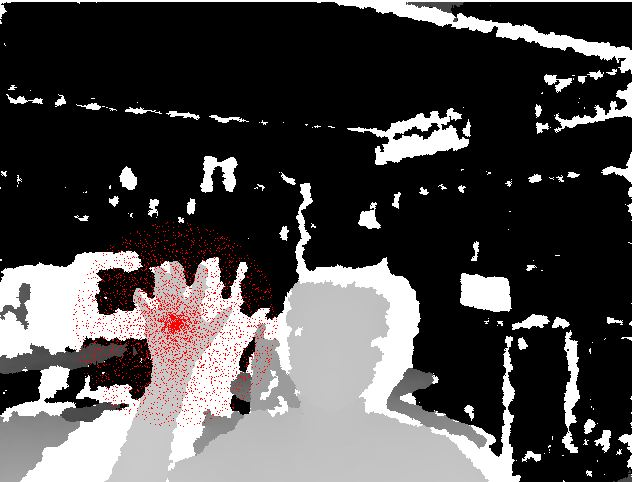
\includegraphics[width=0.23\textwidth]{fig/OpenHandNearOffset.jpg}
	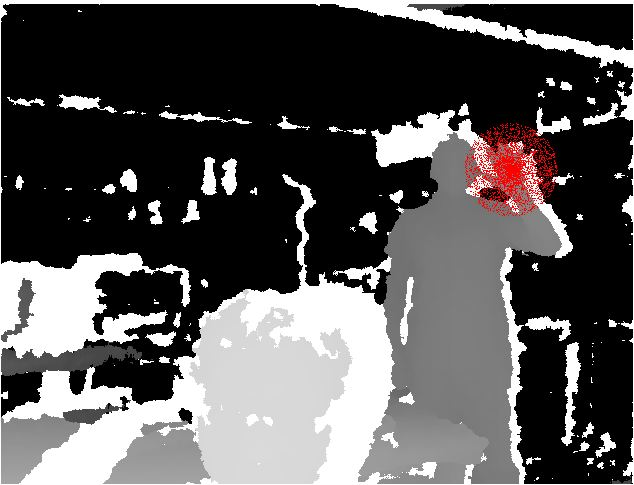
\includegraphics[width=0.23\textwidth]{fig/OpenHandFarOffset.jpg}
	
	\caption{Offset pairs for a given pixel. In the left figure, the reference pixel is the center of the palm. In the right figure, the reference pixel is the center of the palm of the person that stands. }
	\label{fig:offset}
\end{figure}

This feature extraction method is also used by \cite{shotton2011}. The offsets $\theta=\{\bf{u}, \bf{v} \}$ are obtained randomly. In our design, we make those offsets to be uniformly sampled from a bounded circular area. As we can see from Figure \ref{fig:offset}, the offset pairs are located within the neighborhood of the palm and it adaptive to the depth.  
[DO WE NEED MORE EXPLANATION]



\subsection{Training classifier}
We trained the classifier on different subsets of the 400 training samples to study the effect of the training sample size. Also, we set aside 50 samples for testing purposes. Because our prediction is at the pixel level, we sample 1000 pixels from each of the training image, trying to get a good balance between the background and the gesture.

We used a depth-invariant feature vector for each pixel in our training sample. Each feature in the feature vector is the difference in the depth value of two offset pixels from the current pixel. We experimented with different number of such offset pairs for the feature vector.

We trained two classifiers - an SVM classifier for baseline testing, and a random forest classifier with multiple configurations. The random forest classifier can have multiple trees. We explored the effect of different number of trees in the forest.

\subsection{Prediction}
We aimed for real-time prediction of the hand gesture. The trained model from the classifier is used for per-pixel classification. That is, each pixel is classified as belonging to one of the four gestures or to the background. From here we have to first identify the likely gesture, and then find the location of that gesture, a process we called `pooling'. 

\subsubsection{GPU} Running the prediction algorithm using the CPU proved to be very slow. For a $640\times480$ image, our system took 2.5 minutes to classify all the pixels. Given that this problem is highly parallelizable, we turned to the GPU. Re-implementing the prediction algorithm with the GPU reduced the prediction time from 2.5 minutes to 400 milliseconds - a 99.7\% speedup!


\subsection{GPU performance enhancements}